\documentclass[oneside, DIV=11]{scrreprt}
\usepackage[utf8]{inputenc}
\usepackage{graphicx}

\usepackage{gensymb} % Pour le symbole degré

\usepackage[pdftex=true,hyperindex=true,linktocpage=true]{hyperref} % Pour les liens actifs dans le docs

% Pour les en-têtes et les pieds de page
\usepackage[]{fancyhdr}
\pagestyle{fancyplain}
\fancyhf{}
\fancyhead[L]{
\includegraphics[width=2cm]{img/text.png}}
\fancyhead[C]{Specifications}
\fancyhead[R]{\thepage/\pageref{LastPage}}

\fancyfoot[L]{The 2016 Hackaday Prize - Platform D}
\fancyfoot[R]{Alain Sanguinetti}
\renewcommand{\headrulewidth}{0pt}

\usepackage[english]{babel}

\title{Specifications of Platform D}
\author{}
\date{\today}

\begin{document}

\begin{titlepage}
    \begin{flushleft}
        {\sfb
            
\includegraphics[height=1cm]{img/text} \\[7cm]

            {\huge Platform D}\\[.5cm]
            {\LARGE Specifications }\\[.5cm]
            
            % A enlever :!!!!!!!!
            % ##########################################
            %{\large Version préliminaire }\\[2cm]
            % ##########################################
            
        }
        
        
        \vfill
        \emph{Alain Sanguinetti}\\
        \emph{The 2016 Hackaday Prize}
    \end{flushleft}
\end{titlepage}

\tableofcontents
\newpage

\chapter{Introduction}

\section{Projet}


\section{Contexte}



\section{Enoncé du besoin}

\chapter{Objectifs et contraintes techniques}

\section{Analyse fonctionnelle}
Nous avons considéré le système en situation dans une salle d’opération.
L’analyse est représentée sur le graphe des interacteurs (figure \ref{f1}).

\begin{figure}[h]
\centering
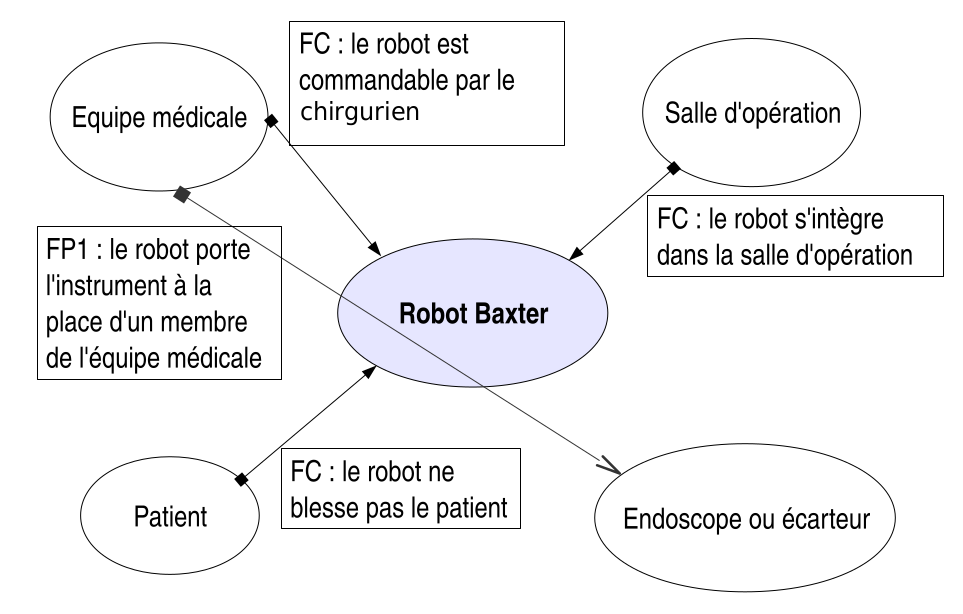
\includegraphics[width=0.85\textwidth]{img/grin2.png}
\caption{Graphe des interacteurs. FP: Fonction principale, FC: Fonction contrainte.}
\label{f1}
\end{figure}

Le détails des critères de chaque fonction est donné ci-dessous.


\section{Fonction principale : “le robot manipule l'instrument à la place d'un membre de l'équipe médicale”}

\begin{itemize}
    \item Les instruments sont installés par l'équipe médicale sur le robot.
    \item A l'aide de la comanipulation, l'équipe médicale rentre un instrument fixé au poignet du robot dans le trocart. 
    \item Le robot peut sortir l'instrument manipulé d'un trocart tout seul mais ne peut pas rentrer d'instrument dans un trocart.
     \item Il existe une procédure pour définir le centre du trocart.
    \item Le système déplace l’endoscope de manière à faire défiler l’image de l’endoscope vers la gauche, la droite, le bas et le haut, l'avant et l'arrière. Les mouvements sont représentés sur la figure \ref{mouvements}, à la page \pageref{mouvements}.
    \item Il existe une procédure pour définir le positionnement du repère de l'instrument.
    \item Les instruments utilisables sont l'endoscope, le même modèle que celui de l'ISIR, et un écarteur, les modèles utilisés pour les opérations par B. Gayet et D. Fuks. \item L'instrument peut être maintenu en position jusqu'à 8h d'affilées dans une salle d'opération où la température est inférieure à 20 \degree C.
    \item Le poignet a une vitesse de déplacement maximale de 25 cm/s.
     %\item Le volume de l'espace de travail dans l'abdomen est ( \underline{à reprendre de la doc Jaimi} ). % Commenté car défini mathématiquement par l'enfoncement de l'endoscope et le trocart.
    \item Le système de fixation de l'instrument est conçu pour être stérile ou est stérilisable par une enveloppe stérile.
    \item L'ensemble réalisé : Baxter, porte-instrument, système de commande n’est pas stérile.
\end{itemize}

\begin{figure}[h]
\centering
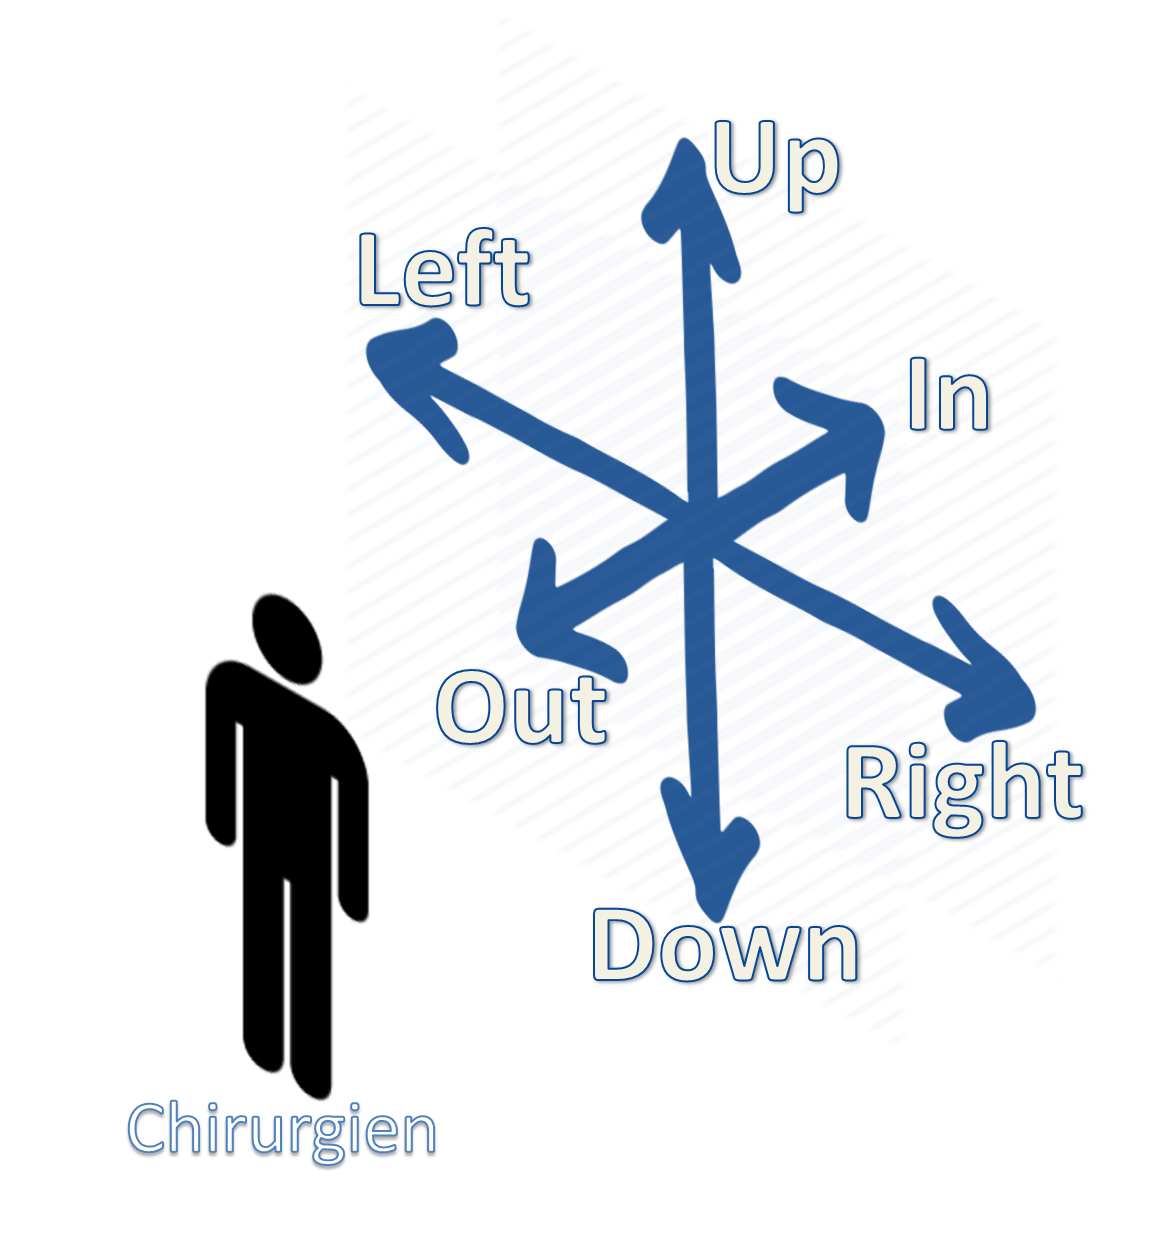
\includegraphics[width=0.50\textwidth]{./img/schema.png}
\caption{Représentation des mouvements possibles de l'extrémité de l'endoscope}
\label{mouvements}
\end{figure}



\section{Fonction contrainte : “le robot est commandable par le chirurgien”}

\begin{itemize}
 \item Le chirurgien peut commander le robot par comanipulation. Dans ce mode de commande, le robot compense son propre poids.
 \item Le chirurgien commande le robot par la voix ou par une pédale.
 \item Dans le cas où l'équipe médicale déclenche un état d'arrêt, le robot arrête son mouvement et s'immobilise.
 \item Un deuxième arrêt d'urgence permet de couper l'alimentation de tous les actionneurs du robot. Dans ce cas, le robot tombe sous l'effet des forces mécaniques. Ce comportement n'est pas acceptable mais la modification du robot Baxter est hors du cadre de ce projet.
 \item L'écran du robot affiche l'image issue de l'endoscope.
\end{itemize}

\section{Fonction contrainte : “le robot s'intègre dans la salle d'opération”}
\begin{itemize}
    \item Un scénario d'habillage du robot est proposé avec des enveloppes stériles standards.
    \item L'espace de travail maximum autorisé est l'espace entre deux plans horizontaux définis par le chirurgien.
    \item Le robot ne nécessite pas d'ordinateur externe.
    %\item Le robot peut surveiller et alerter en cas de mouvement du lit.
    \item Le robot arrête son mouvement en cas de collision entre ses composants externes et un objet ou un humain dans la salle d'opération.
    %\item Le robot précise le lieu de la collision.
    \item A la fin du projet, une évaluation de la de compatibilité électromagnétique est effectuée avec plusieurs instruments, par exemple une pince monopolaire.

\end{itemize}

\section{Fonction contrainte : “le robot ne blesse pas le patient”}
\begin{itemize}
 %\item Le robot ne donne pas de retour d'effort (trop compliqué).
 \item Le robot ne déplace pas les trocarts.
 \item Le diamètre intérieur minimum des trocarts utilisés pour l'endoscope est de 10 mm.
 \item Le diamètre intérieur minimum des trocarts utilisés pour l'écarteur est de 5 mm.
 \item La longueur des trocarts est variable.

\end{itemize}



\chapter{Ressources du projet}

\section{Equipe}
3 étudiants en 4ème année de Robotique à Polytech Paris-UPMC :
Sara Lakhal, Eder Jimenez, Alain Sanguinetti.

\section{Budget}
Le projet ne dispose pas de ressources financières spécifiques. Les clients peuvent acheter du matériel pour le projet. Le matériel est leur propriété.

\section{Temps}
8h par semaine, chaque vendredi jusqu’au 6 juin.
Du 1 au 3 juin, les journées sont libérées pour effectuer les tests du système.


% La partie qui concerne le planning
\chapter{Calendrier}

    \section{5 décembre 2014 : dossier de conception préliminaire}
    
    Le dossier détaillera les choix technologiques généraux.
    
    \section{16 janvier 2015 : bilan de fin de semestre}
    
    A cette date, nous présenterons l'état d'avancement de notre projet.
    
    Le système de fixation des instruments sera complètement concu et défini. Si possible réalisé.
    
    Le robot pourra afficher le flux vidéo issu d'un endoscope sur son écran.

    \section{20 février 2015 : dossier de conception détaillée}
    
    Le dossier présentera le système réalisé de manière précise.
    
    \section{27 mars 2015 : espace de travail}
    
    Une étape intermédiaire de la réalisation du projet sera la possiblité de définir les deux plans horizontaux qui représentent l'espace de travail. Dans cet espace, la comanipulation sera possible. Les dispositifs de commandes seront fonctionnels.

    \section{22 mai 2015 : prototype fonctionnel}

    Les fonctionnalités de calibrage, entrée-sortie d'un trocart et définition d'un trocart seront disponibles.
    
    Le système est fonctionnel, il est possible de lui faire passer des tests.

    \section{3 juin 2015 : fin des tests et fin du projet}
    
    Du 1 au 3 juin nous effectuerons une campagne de tests pour valider le système.
    Le 3 juin, vous êtes invités à assister à la soutenance du projet.


% La page pour les signatures
\label{LastPage}

\end{document}
